\documentclass[conference]{IEEEtran}

\usepackage[utf8]{inputenc}
\usepackage[T1]{fontenc}
\usepackage[spanish, es-nodecimaldot]{babel}

\usepackage{amsmath}
\usepackage{amssymb}
\usepackage{array}
\usepackage{booktabs}
\usepackage{multirow}

\usepackage{graphicx}
\graphicspath{{figures/}}

\usepackage{url}
\usepackage{cite}

\spanishdecimal{.}

\begin{document}

\title{Análisis Agroclimático y Tipologías de Cultivo en el Perú mediante un Enfoque Multi-distrito y \textit{Clustering} no Supervisado (2020--2025)}

\author{
\IEEEauthorblockN{Johao Mendoza, Joyssie Rivas, Thiago Ormeño}
\IEEEauthorblockA{\textit{Departamento de Ingeniería} \\
\textit{Universidad del Pacífico} \\
Lima, Perú \\
\{jr.mendozaf@alum.up.edu.pe, ja.rivasr@alum.up.edu.pe, tc.ormenof@alum.up.edu.pe\}}
}

\maketitle

\begin{abstract}
Este estudio analiza la relación entre variables climáticas y producción agrícola en seis regiones del Perú (Ica, Junín, La Libertad, Piura, Puno y San Martín) durante 2020--2025, integrando producción mensual del MIDAGRI con variables climáticas de NASA POWER bajo la metodología CRISP-DM. Debido a la heterogeneidad ecológica intra-regional, se implementó una estrategia multi-distrito basada en 14 unidades representativas por piso ecológico. La producción mensual fue recuperada desde los acumulados oficiales mediante diferenciación temporal y manejo explícito de datos faltantes. El análisis exploratorio muestra que los determinantes climáticos varían según el piso ecológico: la radiación domina en costa, la humedad de suelo y temperatura máxima en sierra y altiplano, y la humedad relativa en selva. La sequía altoandina de 2022 redujo la producción de quinua ($-64\%$) y oca ($-62\%$) en Puno, mientras que el Fenómeno del Niño 2023--2024 produjo anomalías diferenciadas (Piura $+121\%$ de precipitación). Como fase de modelado, se aplicó \textit{clustering} no supervisado (KMeans, jerárquico Ward, DBSCAN) sobre los perfiles agroclimáticos. Se demuestra, mediante el Índice de Rand Ajustado (ARI), que el clustering ingenuo sobre perfiles región--cultivo reproduce la geografía (ARI $=0.59$ con la región) en lugar de tipificar cultivos, debido a la degeneración de las \textit{features} climáticas. Se proponen y validan dos modelos corregidos: tipologías agroclimáticas territoriales y tipologías de patrón productivo independientes de la geografía (ARI $=0.06$). Los resultados validan el enfoque multi-distrito y aportan una metodología reproducible de caracterización agroclimática.
\end{abstract}

\begin{IEEEkeywords}
Agricultura, cambio climático, NASA POWER, MIDAGRI, análisis agroclimático, piso ecológico, ENSO, CRISP-DM, clustering, KMeans
\end{IEEEkeywords}

\section{Introducción}
La agricultura representa el 4.8\% del PBI peruano en 2025 \cite{bcrp2025} y emplea aproximadamente 4.3 millones de personas (24\% de la PEA) \cite{inei2024}. Las agroexportaciones crecieron de USD 7,791 millones en 2020 a USD 15,066 millones en 2025 \cite{adex2026}. La producción exhibe alta variabilidad por eventos climáticos (sequías, heladas, El Niño) cuya relación con los rendimientos por cultivo no ha sido analizada sistemáticamente con técnicas de \textit{Data Mining} a granularidad mensual.

La complejidad metodológica del análisis agroclimático en el Perú es estructural: las regiones son ecológicamente heterogéneas (una sola región puede combinar costa, sierra y selva), y los datos públicos de producción del MIDAGRI se reportan a nivel regional acumulado, no por piso ecológico ni a granularidad mensual directa. Trabajos previos enfrentan estas limitaciones usando agregados anuales \cite{senamhi2009, unap2016}, asumiendo un único punto climático por región, o restringiéndose a un solo cultivo. La presente investigación combina cuatro aportes: (i) recuperación de producción mensual desde los acumulados publicados; (ii) muestreo climático multi-distrito por piso ecológico; (iii) integración cultivo--piso con criterio agronómico documentado; y (iv) una fase de modelado no supervisado que tipifica el agro peruano y expone un sesgo metodológico habitual en el \textit{clustering} agroclimático.

El objetivo general es caracterizar la relación entre variables climáticas y producción agrícola en seis regiones del Perú bajo la metodología CRISP-DM \cite{inia2019}. Los objetivos específicos son:
\begin{enumerate}
    \item Construir un dataset integrado clima--producción a granularidad cultivo--piso.
    \item Identificar los determinantes climáticos por región y piso ecológico.
    \item Detectar patrones de vulnerabilidad y estacionalidad por cultivo.
    \item Validar la utilidad del enfoque multi-distrito mediante la sequía altoandina 2022 y el Fenómeno del Niño 2023--2024.
    \item Construir tipologías agroclimáticas y de patrón productivo mediante \textit{clustering} no supervisado, evaluando críticamente su validez interna e interpretabilidad.
\end{enumerate}

\section{Estado del Arte}
Diversos estudios han analizado la relación entre variabilidad climática y producción agrícola en el Perú, especialmente frente a eventos ENSO, sequías y cambios de temperatura y precipitación. Restrepo et al. \cite{restrepo2017} evidenciaron que eventos extremos de El Niño alteran significativamente patrones ambientales e hidrológicos en Sudamérica, afectando sistemas agrícolas vulnerables. Asimismo, estudios nacionales destacan diferencias agroclimáticas entre costa, sierra y selva debido a la heterogeneidad ecológica del territorio peruano.

En paralelo, el uso de metodologías de \textit{Data Mining} y CRISP-DM en agricultura ha crecido en los últimos años. Chapapría y Viladrich \cite{chapapria2024} desarrollaron un modelo agroclimático basado en CRISP-DM, mientras que Canchano \cite{canchano2024} aplicó técnicas predictivas para productos agrícolas. Sin embargo, estos enfoques se centran principalmente en tareas predictivas y presentan limitaciones en la integración espacial y temporal de datos.

Por otro lado, trabajos de zonificación agroecológica desarrollados por MIDAGRI \cite{midagri2025} y la Universidad Nacional del Altiplano \cite{una2023} resaltan la importancia de considerar pisos ecológicos en estudios agrícolas. No obstante, gran parte de la literatura emplea agregados anuales, análisis de un solo cultivo o un único punto climático por región, limitando la representación de microclimas y dinámicas intra-regionales. En particular, el \textit{clustering} agroclimático suele aplicarse sin auditar si la partición resultante captura información productiva o si simplemente reproduce la estructura geográfica de los datos, vacío metodológico que este trabajo aborda explícitamente.

En consecuencia, persiste un vacío en la integración de producción agrícola mensual, variables climáticas multi-distrito y caracterización agroecológica mediante minería de datos para múltiples regiones peruanas.

\section{Metodología}

\subsection{Fuentes de datos y variables}
Se adoptó la metodología CRISP-DM \cite{chapman2000} en sus fases de comprensión del negocio, comprensión y preparación de datos, modelado y evaluación. Se integraron dos fuentes públicas: (i) la hoja \texttt{c-18} de los reportes mensuales del MIDAGRI \cite{midagrihist}, con producción acumulada por región, mes y cultivo para 2020--2025; y (ii) variables agroclimáticas de NASA POWER \cite{nasa2025}. Las variables climáticas fueron seleccionadas por su relevancia sobre fenología, disponibilidad hídrica y rendimiento \cite{viladrich} (Tabla~\ref{tab:variables}).

\begin{table}[h]
\centering
\caption{Variables climáticas seleccionadas (NASA POWER)}
\label{tab:variables}
\small
\begin{tabular}{l l}
\toprule
\textbf{Variable} & \textbf{Descripción} \\
\midrule
T2M & Temperatura media \\
T2M\_MAX / T2M\_MIN & Temperatura máxima / mínima \\
PRECTOTCORR & Precipitación corregida \\
RH2M & Humedad relativa \\
ALLSKY\_SFC\_SW\_DWN & Radiación solar superficial \\
GWETROOT & Humedad de suelo (zona radicular) \\
\bottomrule
\end{tabular}
\end{table}

\subsection{Recuperación y calidad de los datos}
La hoja \texttt{c-18} reporta producción acumulada anual y no mensual directa. La producción mensual se recuperó mediante diferenciación entre meses consecutivos:
\begin{equation}
Prod_{m} = Acum_{m} - Acum_{m-1}
\end{equation}

Tres meses no publicados por MIDAGRI (dic-2020, may-2021 y mar-2022) fueron incorporados como valores faltantes explícitos antes del cálculo de diferencias para evitar sobreestimaciones. Diciembre 2020 se recuperó a partir del total anual publicado en el archivo de diciembre 2021. La Tabla~\ref{tab:calidad} resume los tratamientos de calidad.

\begin{table}[h]
\centering
\caption{Tratamientos de calidad de datos}
\label{tab:calidad}
\small
\begin{tabular}{p{2cm} p{4.3cm}}
\toprule
\textbf{Caso} & \textbf{Tratamiento} \\
\midrule
Meses faltantes MIDAGRI & NaN explícito y recuperación Dic-2020 \\
Valores \texttt{-999} NASA & Tratados como NaN y estimados con continuidad temporal local \\
Negativos en \texttt{diff()} & Conversión a NaN \\
Ceros estructurales & Conservados \\
Eventos extremos & Conservados como señal \\
\bottomrule
\end{tabular}
\end{table}

No se aplicó remoción de outliers mediante IQR o Z-score debido a la alta presencia de ceros estructurales y a que eventos extremos como la sequía 2022 en Puno \cite{rcr2023} y El Niño Costero 2023--2024 \cite{senamhi2024} constituyen la señal de interés del estudio.

\subsection{Estrategia multi-distrito y construcción de datasets}
Debido a la heterogeneidad ecológica de las regiones peruanas, se seleccionaron 14 distritos representativos distribuidos por piso ecológico para evitar sesgos derivados de un único punto climático regional. La selección consideró especialización agrícola y representatividad agroecológica (Tabla~\ref{tab:distritos}).

\begin{table}[h]
\centering
\caption{Distritos representativos por piso ecológico}
\label{tab:distritos}
\small
\begin{tabular}{l l l}
\toprule
\textbf{Región} & \textbf{Distrito} & \textbf{Piso ecológico} \\
\midrule
Ica & Chincha Alta & Costa \\
La Libertad & Virú & Costa \\
La Libertad & Huamachuco & Sierra \\
La Libertad & Cascas & Yunga \\
Piura & Tambogrande & Bosque seco \\
Piura & Sullana & Valle Chira \\
Piura & Canchaque & Sierra cafetalera \\
San Martín & Moyobamba & Selva Alto Mayo \\
San Martín & Tocache & Selva Huallaga \\
Junín & Perené & Selva alta \\
Junín & Río Tambo & Selva baja \\
Junín & El Tambo & Sierra Mantaro \\
Puno & Ilave & Altiplano lacustre \\
Puno & Ayaviri & Puna alta \\
\bottomrule
\end{tabular}
\end{table}

{\footnotesize Fuente: elaboración propia basada en \cite{redesarrolloica2021, esan2023, cepiura2023, dataperu2021, inei1996, midagripuno2020}.}

Se construyeron tres datasets: (i) un dataset regional agregado por región y distrito; (ii) un dataset clima--producción por cultivo (2{,}376 observaciones cultivo--mes); y (iii) un dataset filtrado mediante Pareto-80, conservando los cultivos que representan el 80\% de la producción regional total (33 combinaciones región--cultivo).

\subsection{Fase de modelado: clustering no supervisado}
Como fase de modelado CRISP-DM se aplicaron tres algoritmos de \textit{clustering} no supervisado: KMeans (partición por minimización de inercia), aglomerativo jerárquico con enlace de Ward, y DBSCAN (densidad). La selección de $K$ se realizó mediante barrido $K=2,\dots,8$ con consenso entre el coeficiente de Silhouette (cohesión vs. separación, mayor es mejor) y el índice de Davies--Bouldin (menor es mejor). Todas las \textit{features} se estandarizaron por $z$-score; para DBSCAN se reportó Silhouette excluyendo los puntos de ruido (etiqueta $-1$).

Para auditar \emph{qué} información captura cada partición se empleó el Índice de Rand Ajustado (ARI) entre las etiquetas de cluster y la región administrativa: un ARI alto indica que el modelo reproduce la geografía, mientras que un ARI bajo indica que el modelo captura estructura distinta (p.~ej.\ patrones productivos). Esta auditoría guió el rediseño del esquema de \textit{features}, descrito en la Sección~\ref{sec:clustering}.

\section{Resultados}

\subsection{Heterogeneidad climática y concentración productiva}
La distribución mensual de temperatura por región y piso (Fig.~\ref{fig:boxplot_temp}) confirma la premisa central del estudio: una misma región administrativa combina pisos térmicamente contrastados. La Libertad, por ejemplo, agrupa costa ($\sim$20\,°C) y sierra ($\sim$11\,°C); Junín combina selva ($\sim$24\,°C), sierra ($\sim$9\,°C) y puna. Esta heterogeneidad invalida el uso de un único punto climático regional y justifica el muestreo multi-distrito.

\begin{figure}[h]
    \centering
    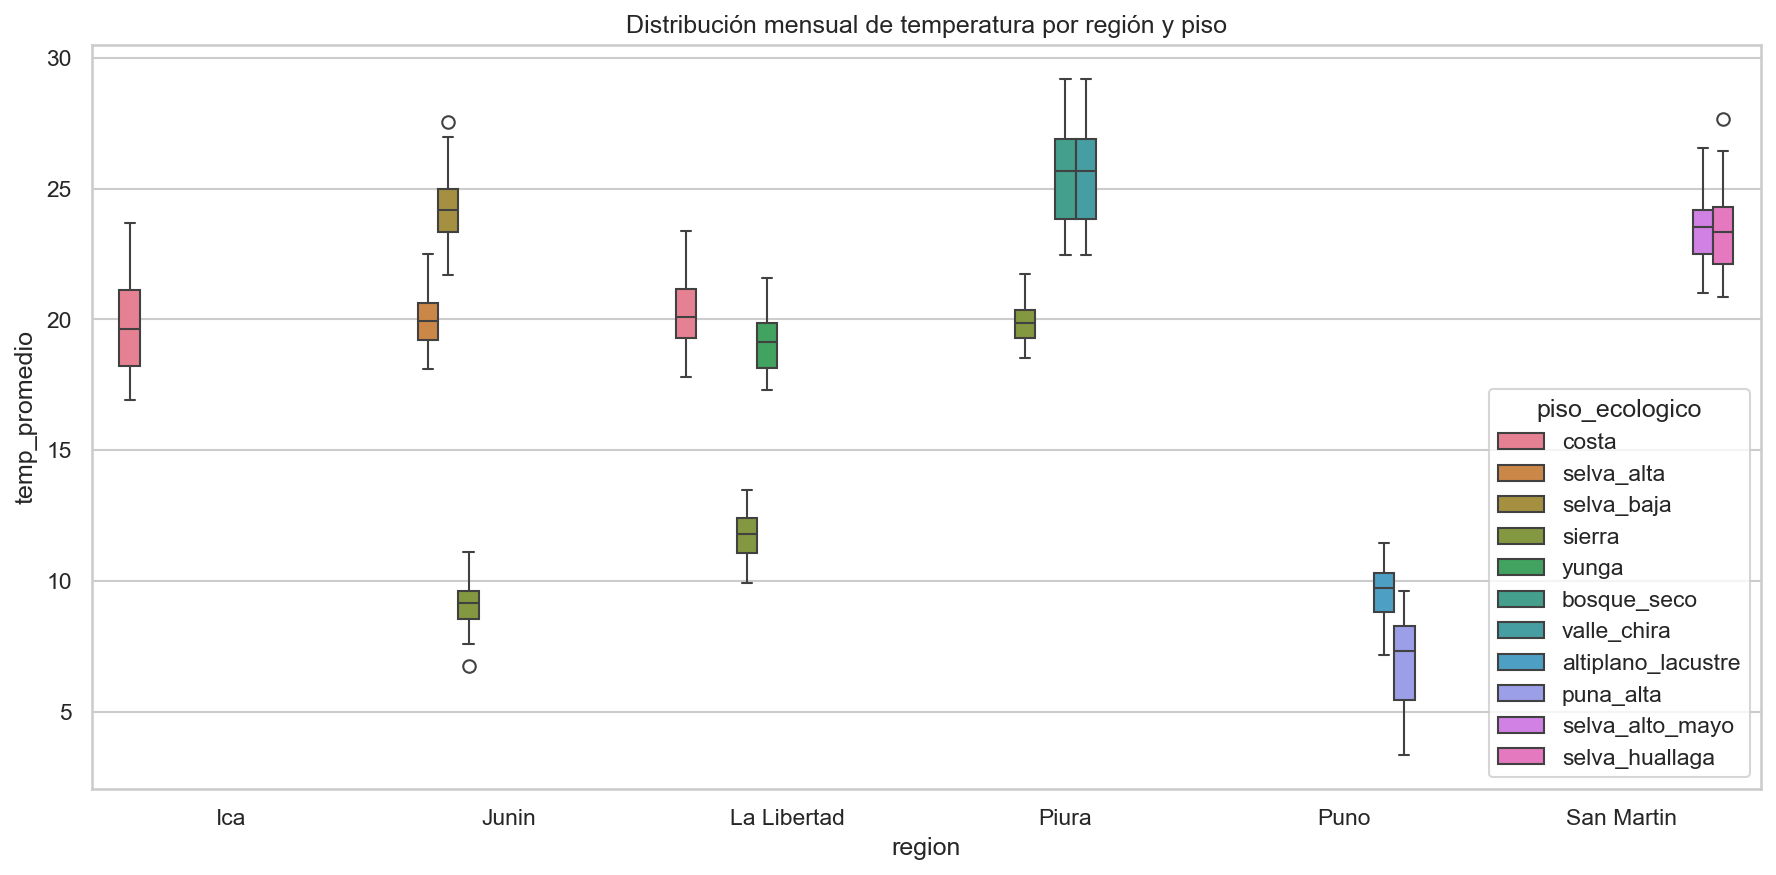
\includegraphics[width=0.48\textwidth]{eda_regional_boxplot_temp.png}
    \caption{Distribución mensual de temperatura por región y piso ecológico. Una misma región combina pisos térmicamente muy distintos.}
    \label{fig:boxplot_temp}
\end{figure}

La producción agregada 2020--2025 muestra fuerte concentración en pocas unidades región--piso (Fig.~\ref{fig:prod_unidad}). La Libertad--Costa (Virú) lidera con 36.84\,M\,tn, dominada por caña de azúcar agroindustrial. Le siguen las unidades altoandinas de Puno: puna alta (Ayaviri, 20.36\,M\,tn) y altiplano lacustre (Ilave, 10.19\,M\,tn), asociadas a avena forrajera y alfalfa. Ica--Costa (Chincha Alta, 9.32\,M\,tn) exhibe el perfil agroexportador más diversificado. El rango entre la unidad más y menos productiva (Cascas--Yunga, 0.36\,M\,tn) abarca dos órdenes de magnitud.

\begin{figure}[h]
    \centering
    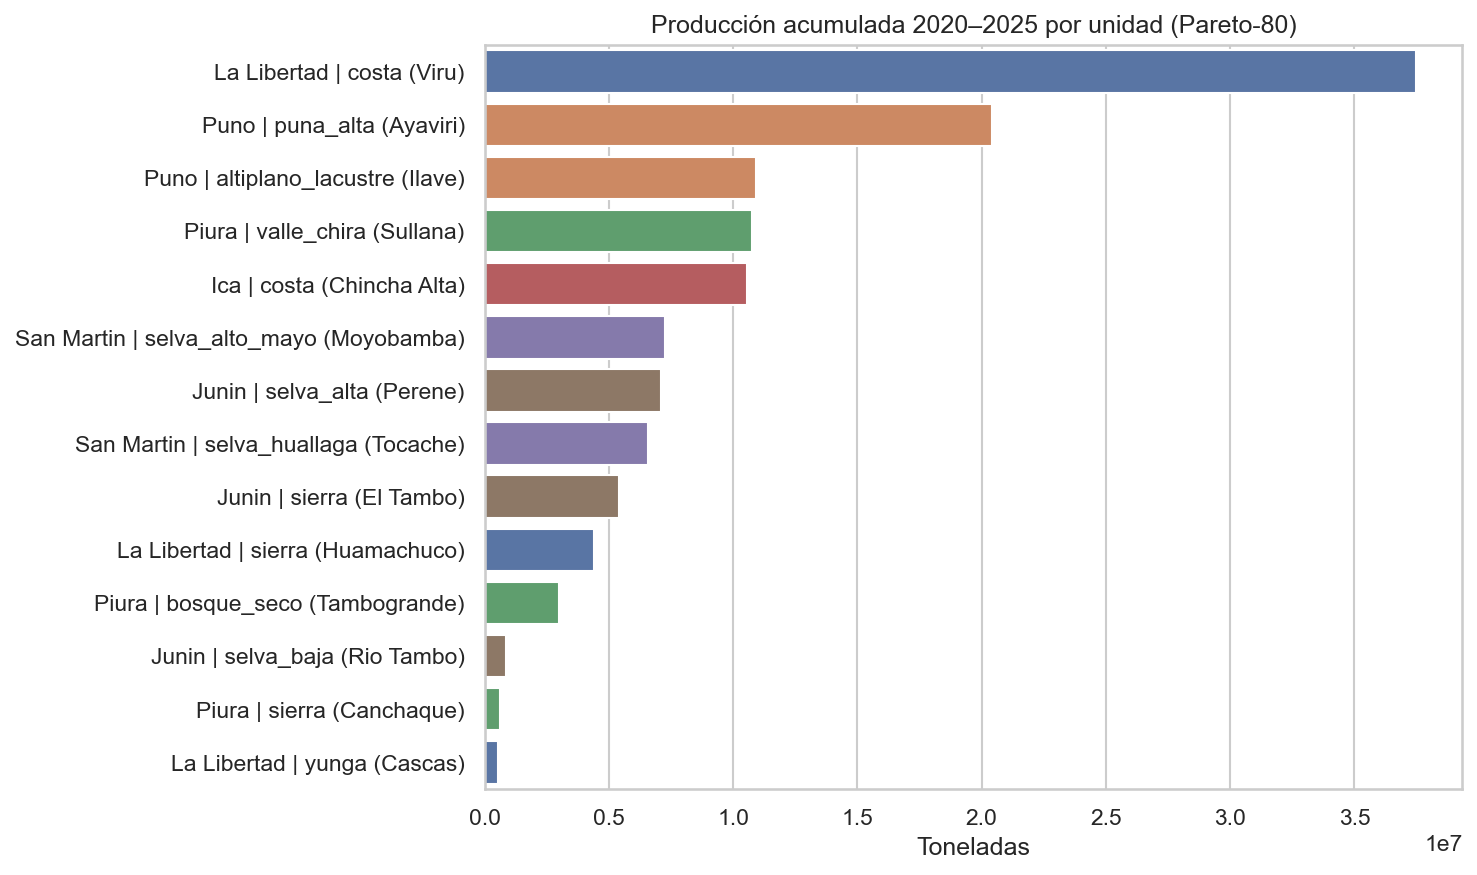
\includegraphics[width=0.46\textwidth]{eda_regional_volumen_unidad.png}
    \caption{Producción acumulada 2020--2025 por unidad región--piso (Pareto-80).}
    \label{fig:prod_unidad}
\end{figure}

El calendario mensual de cosechas (Fig.~\ref{fig:calendario}) revela contrastes de estacionalidad. Las unidades altoandinas de Puno concentran producción entre marzo y mayo, reflejando el ciclo único de cultivos andinos, mientras que La Libertad--Costa e Ica--Costa mantienen producción uniforme durante el año, propia de sistemas agroexportadores intensivos y cultivos perennes. Las unidades de selva presentan estacionalidad intermedia.

\begin{figure}[h]
    \centering
    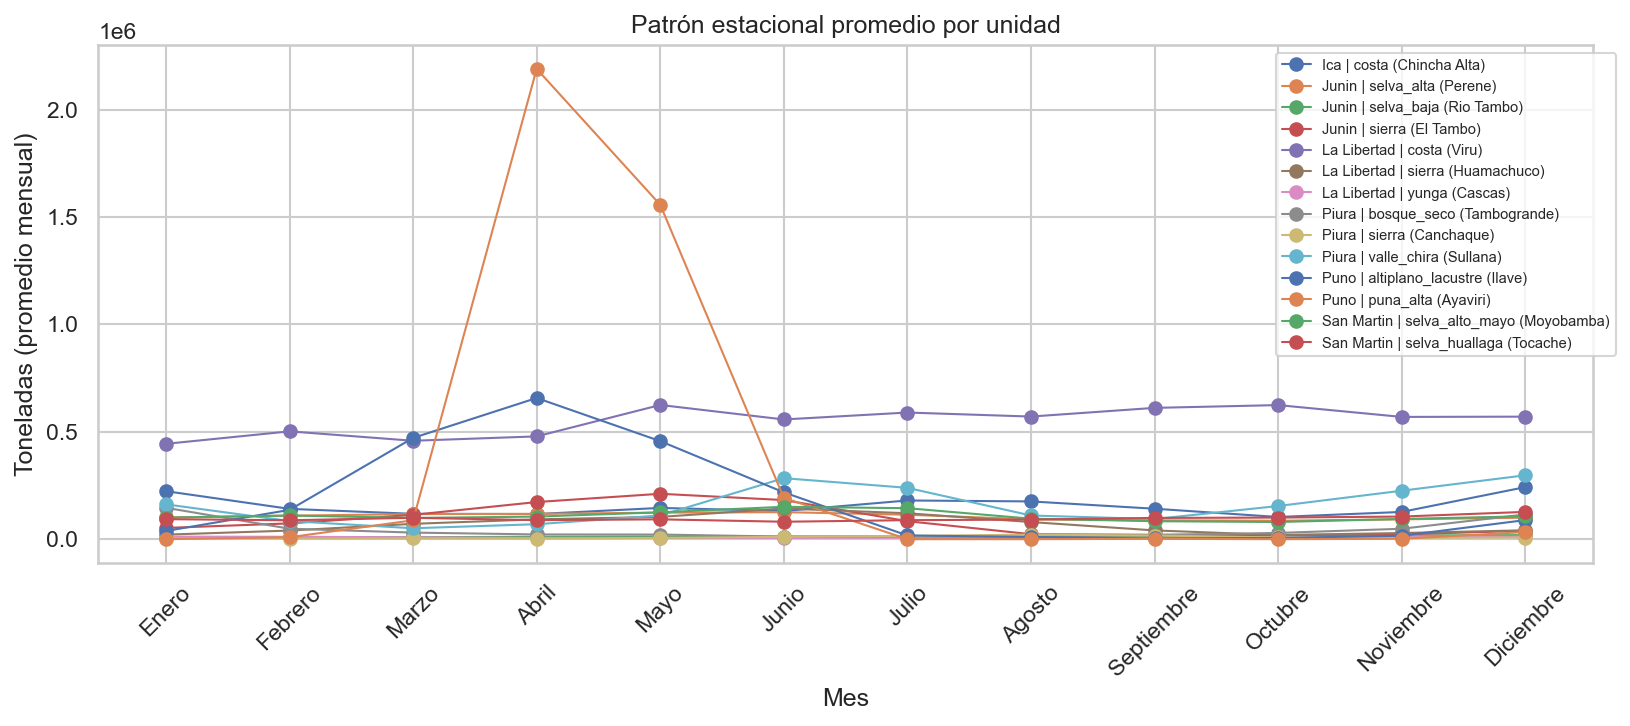
\includegraphics[width=0.48\textwidth]{eda_regional_patron_estacional.png}
    \caption{Patrón estacional promedio por unidad región--piso. La puna alta de Puno concentra su producción en abril--mayo.}
    \label{fig:calendario}
\end{figure}

\subsection{Relaciones clima--cultivo por piso ecológico}
Las correlaciones de Pearson entre producción mensual y clima por cultivo dominante (Fig.~\ref{fig:corr_clima}) muestran patrones coherentes con la fisiología de cada piso. En la costa iqueña, la uva correlaciona positivamente con humedad relativa ($r=+0.62$), radiación ($r=+0.62$) y temperatura mínima ($r=+0.55$). En la selva de Junín, la humedad relativa domina cultivos como piña ($r=+0.76$), que a su vez correlaciona negativamente con radiación ($r=-0.61$). Los cultivos andinos muestran fuerte sensibilidad hídrica y térmica: la alfalfa de Puno depende de la humedad de suelo ($r=+0.66$) y la papa de Junín responde negativamente a la temperatura máxima ($r=-0.52$). Las correlaciones cambian de magnitud y signo entre pisos para variables equivalentes, evidenciando que los agregados regionales ocultan relaciones agroclimáticas relevantes.

\begin{figure}[h]
    \centering
    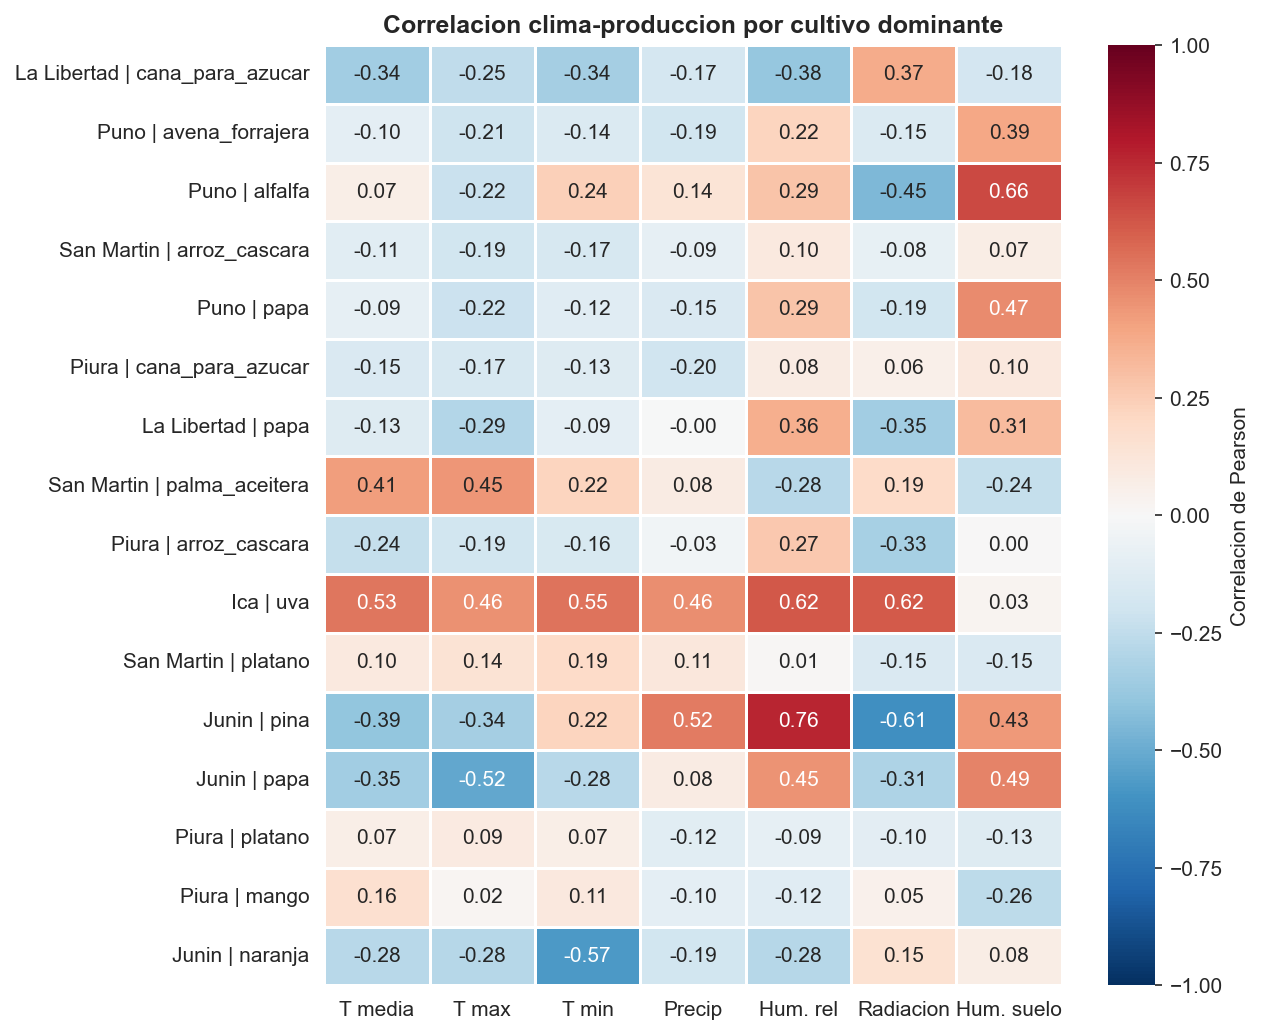
\includegraphics[width=0.48\textwidth]{corr_clima_cultivo.png}
    \caption{Correlación de Pearson entre variables climáticas y producción mensual por cultivo dominante. Las relaciones cambian de signo entre pisos ecológicos.}
    \label{fig:corr_clima}
\end{figure}

\subsection{Eventos climáticos extremos: sequía 2022 y El Niño 2023--2024}
El año 2022 registró en Puno la menor humedad de suelo del periodo (Fig.~\ref{fig:puno_sequia}), con caídas de producción cercanas al 50\% en altiplano lacustre y 37\% en puna alta respecto a 2020. El impacto fue más severo en cultivos andinos tradicionales: quinua cayó 64\%, oca 62\%, cebada forrajera 55\% y papa 47\%, mientras que la avena forrajera mostró mayor resiliencia hídrica, amortiguando la caída agregada. Estos resultados validan la necesidad del análisis desagregado por cultivo.

\begin{figure}[h]
    \centering
    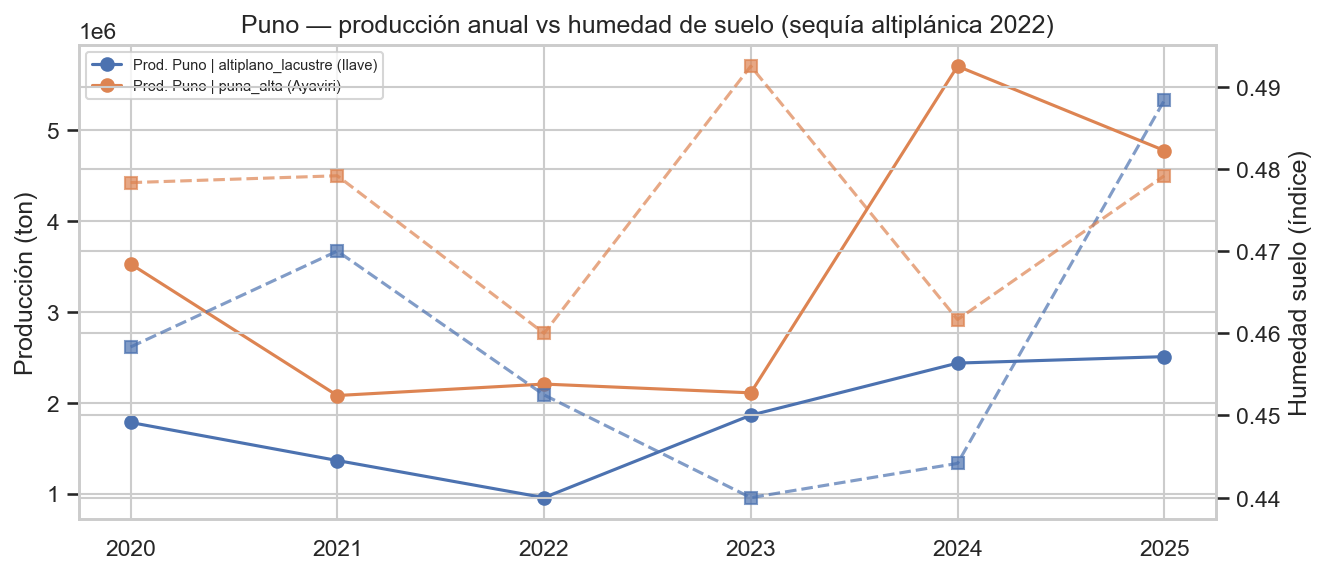
\includegraphics[width=0.46\textwidth]{eda_regional_puno_sequia.png}
    \caption{Producción anual de Puno frente a la humedad de suelo. La sequía de 2022 coincide con el mínimo de humedad y producción.}
    \label{fig:puno_sequia}
\end{figure}

El periodo 2023--2024 registró anomalías consistentes con el Fenómeno del Niño Costero (Fig.~\ref{fig:nino}). Todas las regiones incrementaron su temperatura media entre 4.8\% y 9.2\%. Piura presentó la mayor anomalía de precipitación ($+121\%$), coherente con la intensificación de lluvias en la costa norte reportada por SENAMHI \cite{senamhi2024}, mientras que San Martín redujo su precipitación ($-28\%$) y humedad relativa ($-8.6\%$), evidenciando respuestas regionales diferenciadas.

\begin{figure}[h]
    \centering
    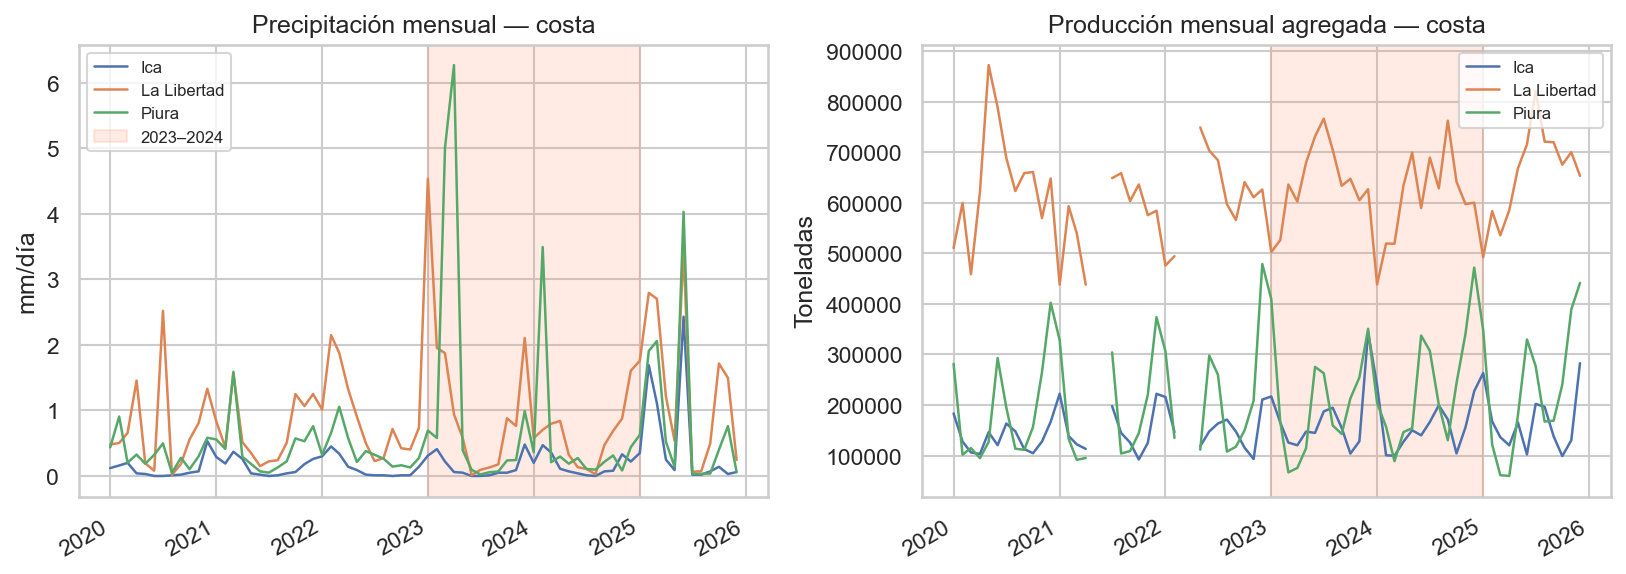
\includegraphics[width=0.48\textwidth]{eda_regional_nino_costa.png}
    \caption{Precipitación y producción mensual en la costa (Ica, La Libertad, Piura). La franja sombreada (2023--2024) marca el Niño Costero, con un pico de lluvias en Piura.}
    \label{fig:nino}
\end{figure}

\subsection{Tipologías agroclimáticas mediante clustering}
\label{sec:clustering}

\subsubsection{Enfoque inicial y diagnóstico crítico}
El primer modelo agrupó los 33 perfiles región--cultivo descritos por 13 \textit{features}: media y desviación estándar de cinco variables climáticas, más producción total, media de cosecha y coeficiente de variación. El barrido de $K$ (Fig.~\ref{fig:seleccion_k}) seleccionó $K=6$ por coincidencia de Silhouette máximo (0.514) y Davies--Bouldin mínimo (0.604). El dendrograma Ward (Fig.~\ref{fig:dendro06}) y el mapa de calor de centroides (Fig.~\ref{fig:heatmap06}) confirman seis grupos bien separados.

\begin{figure}[h]
    \centering
    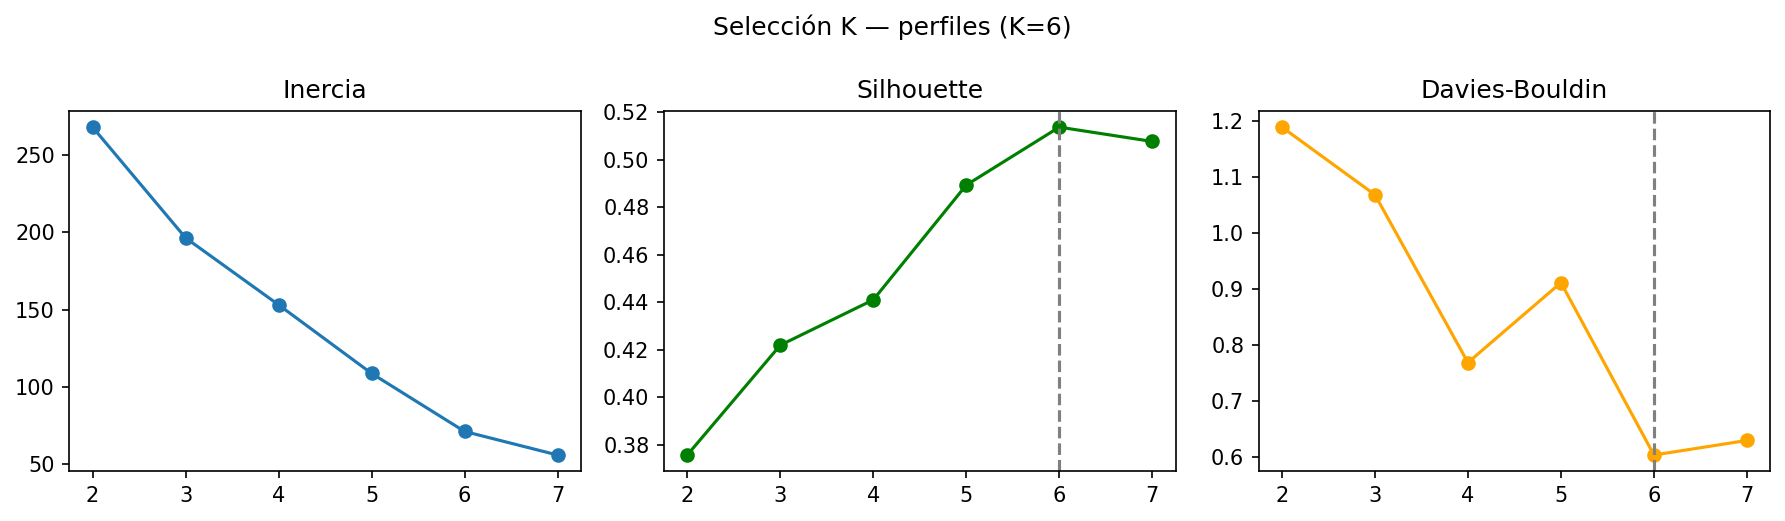
\includegraphics[width=0.48\textwidth]{seleccion_k_perfiles.png}
    \caption{Selección de $K$ para los perfiles región--cultivo: inercia (codo), Silhouette y Davies--Bouldin. El óptimo es $K=6$.}
    \label{fig:seleccion_k}
\end{figure}

\begin{figure}[h]
    \centering
    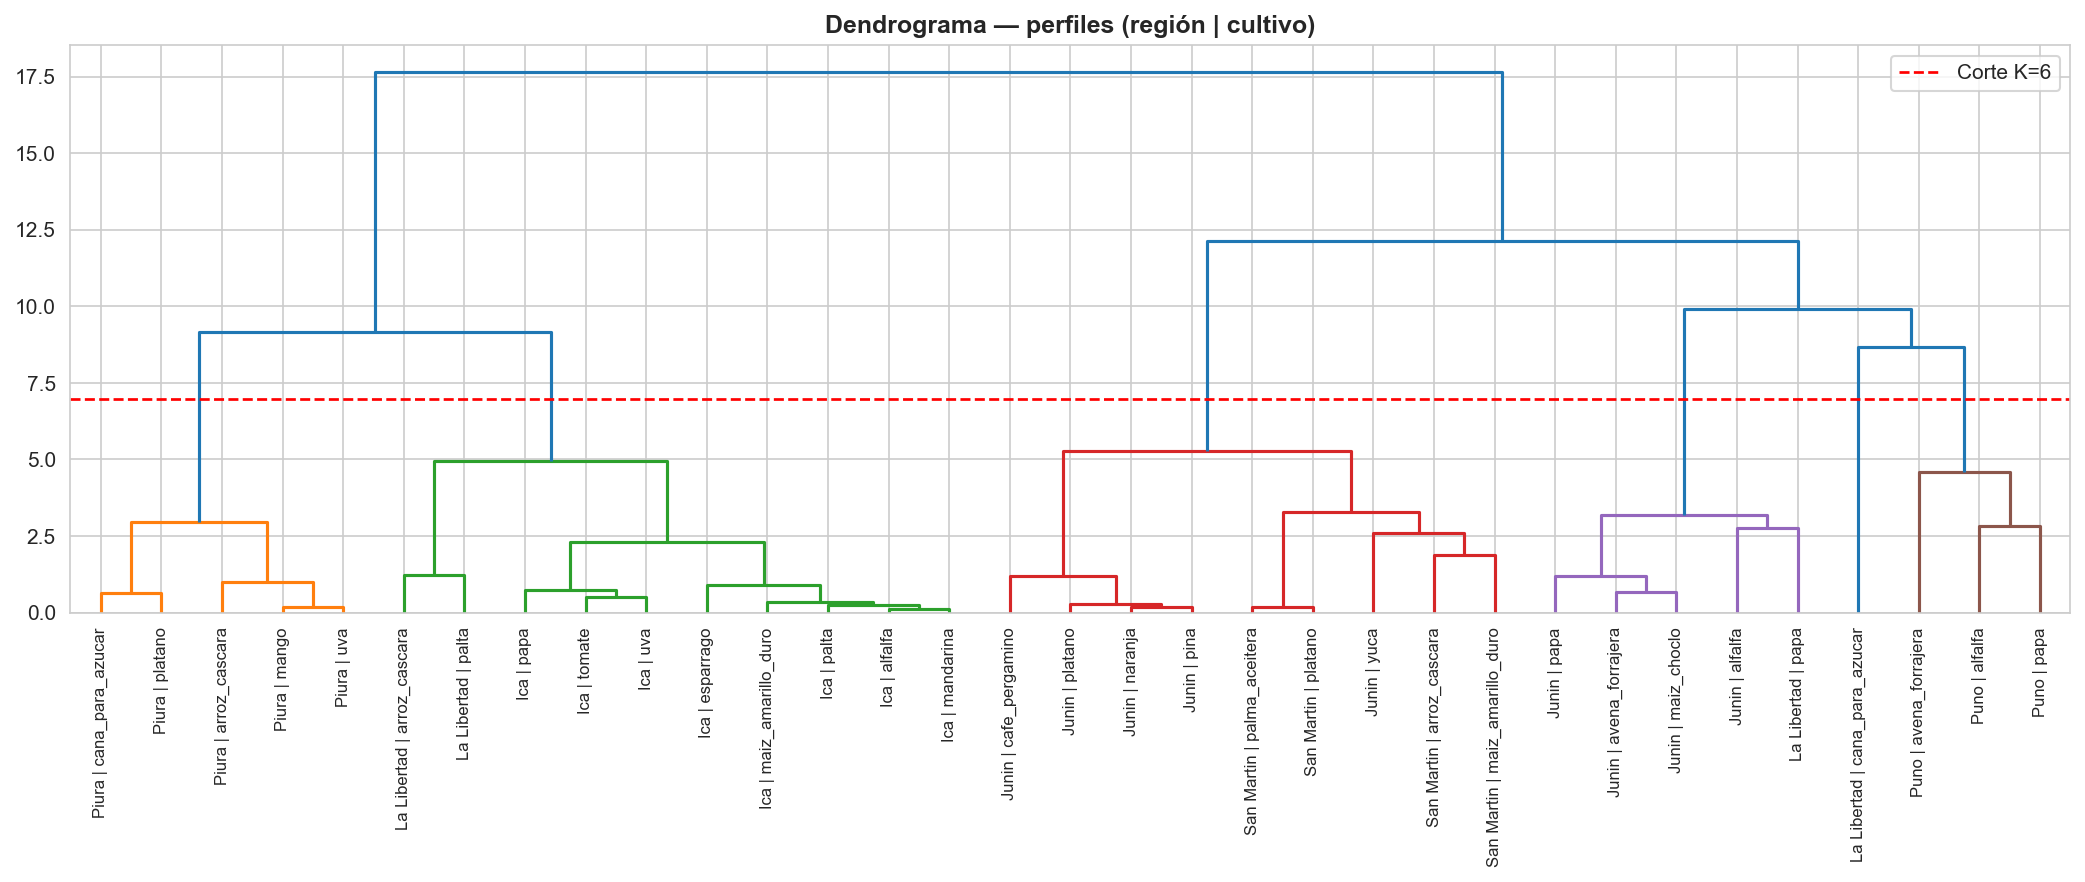
\includegraphics[width=0.48\textwidth]{dendrograma_perfiles.png}
    \caption{Dendrograma Ward de los perfiles región--cultivo. La línea roja indica la altura de corte que produce $K=6$ clusters.}
    \label{fig:dendro06}
\end{figure}

\begin{figure}[h]
    \centering
    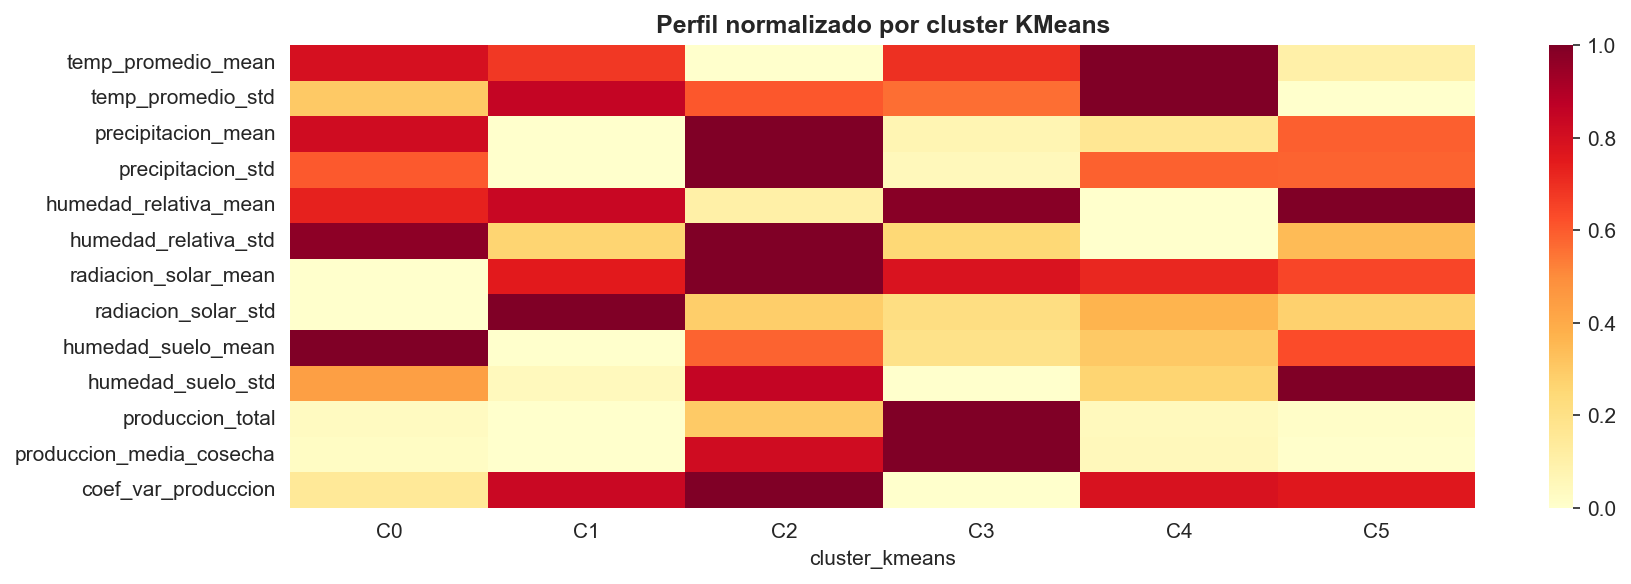
\includegraphics[width=0.48\textwidth]{heatmap_perfiles_kmeans.png}
    \caption{Centroides normalizados (min--max) por cluster KMeans del enfoque inicial. Las \textit{features} climáticas dominan sobre las productivas.}
    \label{fig:heatmap06}
\end{figure}

Sin embargo, una auditoría con el Índice de Rand Ajustado revela un problema de validez: el ARI entre los clusters y la región administrativa es 0.59, y eliminar por completo las variables de producción altera la partición en menos del 20\% de los casos. La causa es una degeneración estructural: dado que el clima es constante por distrito, las 10 \textit{features} climáticas solo toman 11 valores distintos (los distritos) y dominan numéricamente a las 3 \textit{features} productivas. \emph{El modelo no tipifica cultivos: reproduce la geografía}. El Silhouette alto es, en este caso, un artefacto de la redundancia espacial y no evidencia de una tipología agronómica genuina. Este diagnóstico motivó dos rediseños.

\subsubsection{Modelo A --- Tipologías agroclimáticas territoriales}
El primer rediseño asume explícitamente que la unidad real de análisis es la zona climática. Se agruparon las 12 zonas (distritos) usando solo \textit{features} climáticas, y la producción se reservó como variable descriptiva \emph{a posteriori}. El modelo produce $K=5$ tipologías nítidas (Silhouette 0.415, ARI con región 0.40), interpretables sin ambigüedad (Fig.~\ref{fig:heatmap_zonas}): sierra templada, selva húmeda, costa árida, costa norte/bosque seco y altiplano frío. La caracterización productiva \emph{a posteriori} (Fig.~\ref{fig:prod_zonas}) responde la pregunta agronómica ``qué se cultiva en cada clima'': la costa árida concentra caña, uva y palta; el altiplano frío, forrajeras de alto volumen; la selva húmeda, arroz, plátano y palma.

\begin{figure}[h]
    \centering
    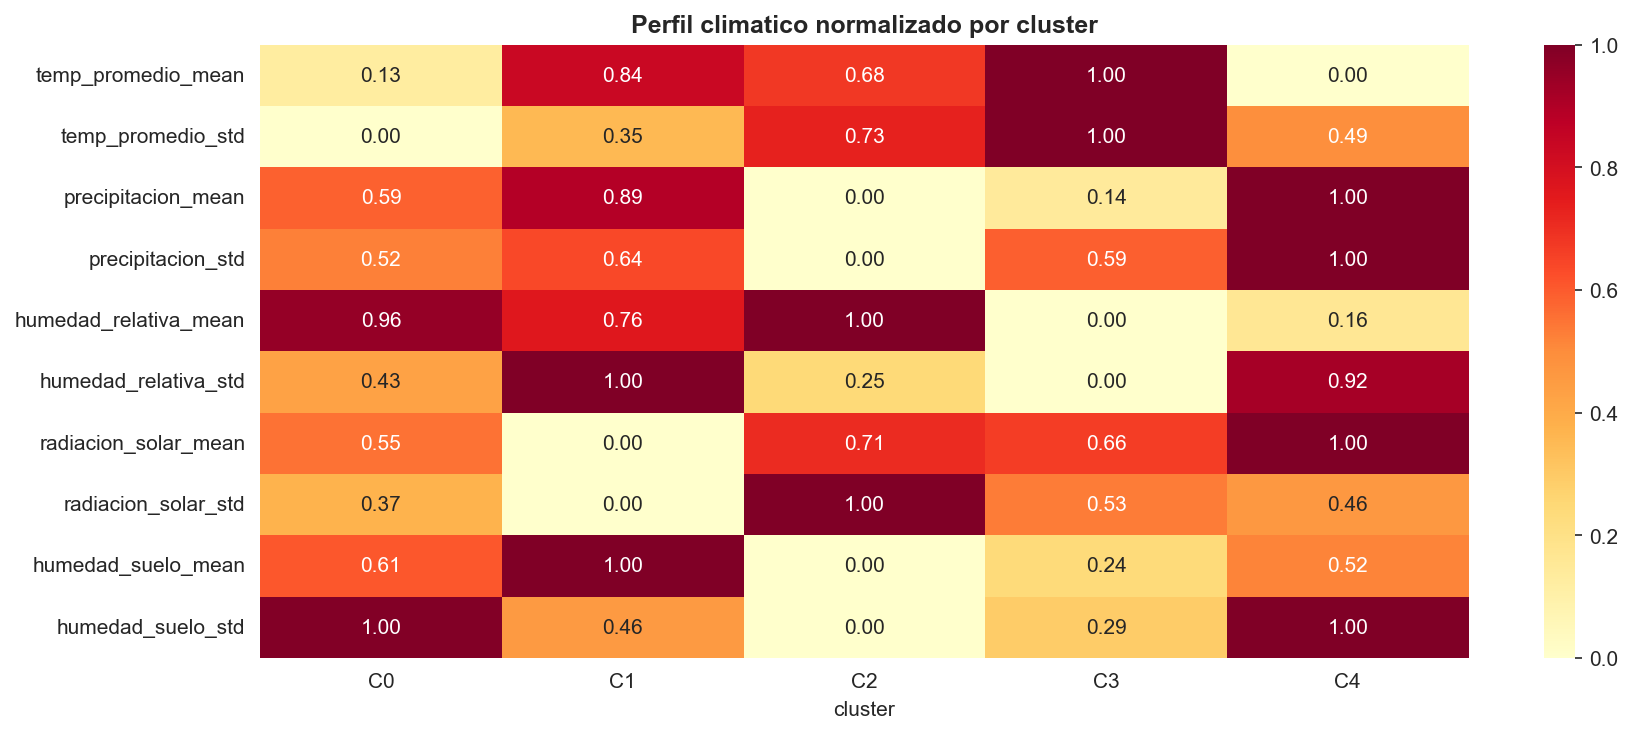
\includegraphics[width=0.48\textwidth]{06a_heatmap_zonas.png}
    \caption{Modelo A: perfil climático normalizado por cluster. Cada columna corresponde a una tipología agroclimática territorial.}
    \label{fig:heatmap_zonas}
\end{figure}

\begin{figure}[h]
    \centering
    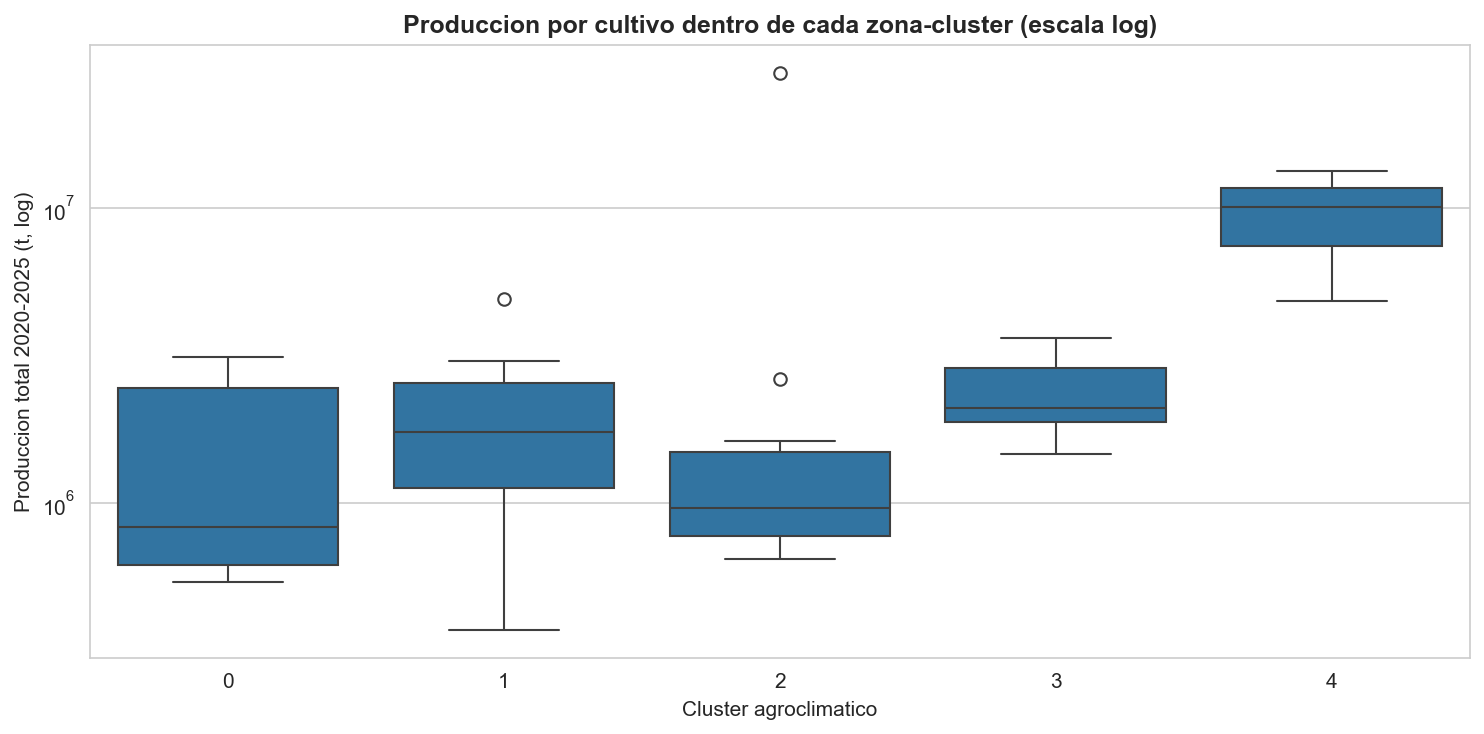
\includegraphics[width=0.46\textwidth]{06a_produccion_por_cluster.png}
    \caption{Modelo A: producción por cultivo dentro de cada zona-cluster (escala log). La producción se usa como descriptor, no como \textit{input}.}
    \label{fig:prod_zonas}
\end{figure}

\subsubsection{Modelo B --- Tipologías de patrón productivo}
El segundo rediseño busca que el cultivo, y no la geografía, determine el agrupamiento. Cada perfil región--cultivo se describió por su \emph{estacionalidad}: un vector de 12 fracciones mensuales de producción (forma del calendario, independiente de la escala), más \texttt{log1p}(producción total), concentración del mes pico, número de meses de cosecha y coeficiente de variación; el clima se redujo a solo 2 componentes principales para evitar que dominara. El transformado logarítmico neutraliza el \textit{outlier} de la caña de Virú.

El modelo produce $K=6$ tipologías de patrón productivo (Fig.~\ref{fig:heatmap_b}) con ARI de apenas 0.06 con la región: el vínculo con la geografía se ha roto. Cultivos de regiones distintas se agrupan por compartir calendario --- por ejemplo, un cluster ``permanente/plano'' reúne espárrago de Ica, caña de La Libertad y de Piura, palma y plátano de selva (concentración mensual $\approx0.08$), mientras que otro cluster agrupa las forrajeras de Puno por su cosecha concentrada en abril--mayo. El dendrograma (Fig.~\ref{fig:dendro_b}) y la proyección PCA (Fig.~\ref{fig:pca_b}) muestran grupos definidos por la forma del ciclo productivo.

\begin{figure}[h]
    \centering
    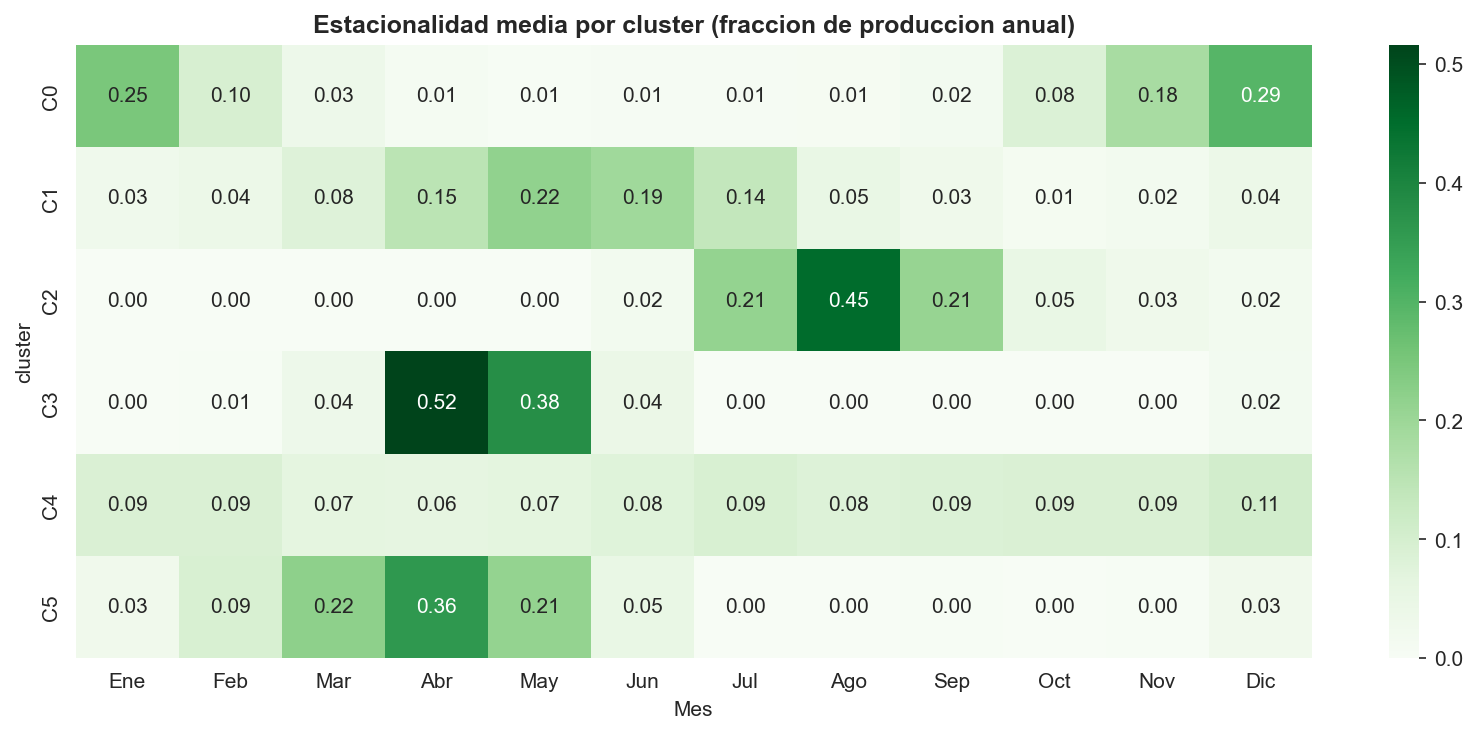
\includegraphics[width=0.48\textwidth]{06b_heatmap_estacionalidad.png}
    \caption{Modelo B: estacionalidad media por cluster (fracción de producción anual por mes). Cada fila es un patrón de calendario productivo.}
    \label{fig:heatmap_b}
\end{figure}

\begin{figure}[h]
    \centering
    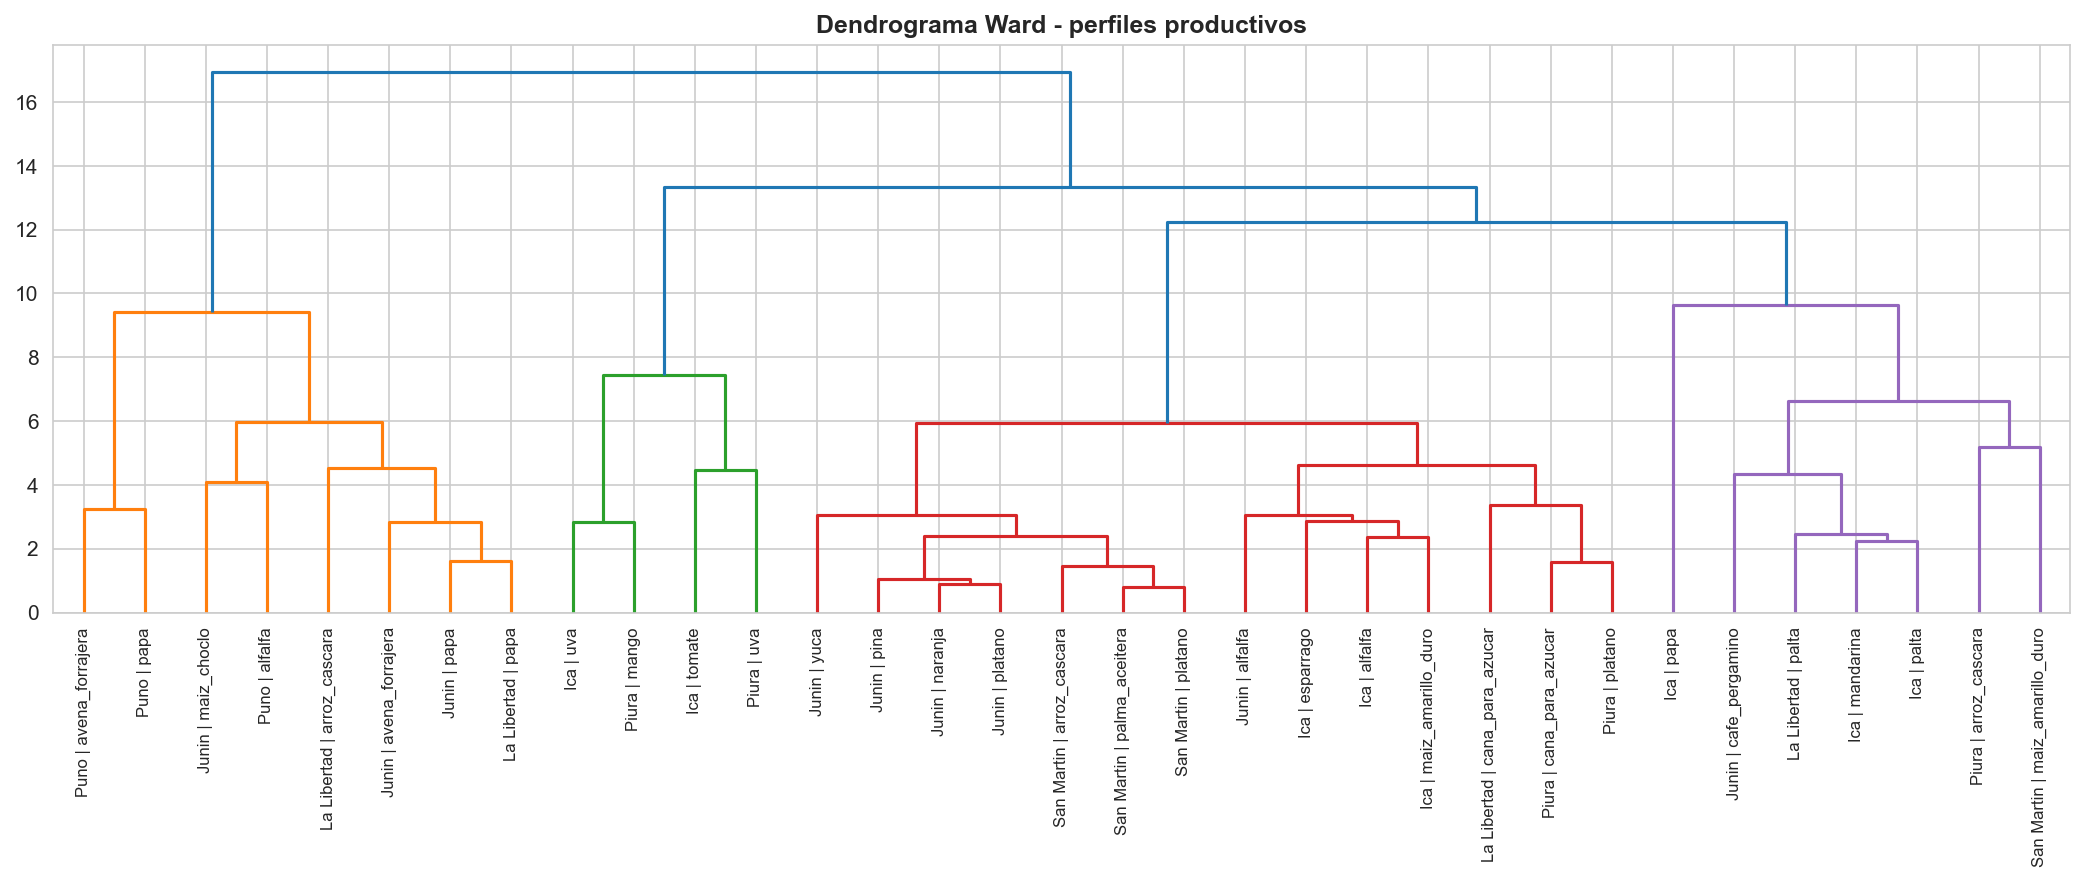
\includegraphics[width=0.48\textwidth]{06b_dendrograma_perfiles.png}
    \caption{Modelo B: dendrograma Ward de los perfiles productivos, con la línea de corte para $K=6$.}
    \label{fig:dendro_b}
\end{figure}

\begin{figure}[h]
    \centering
    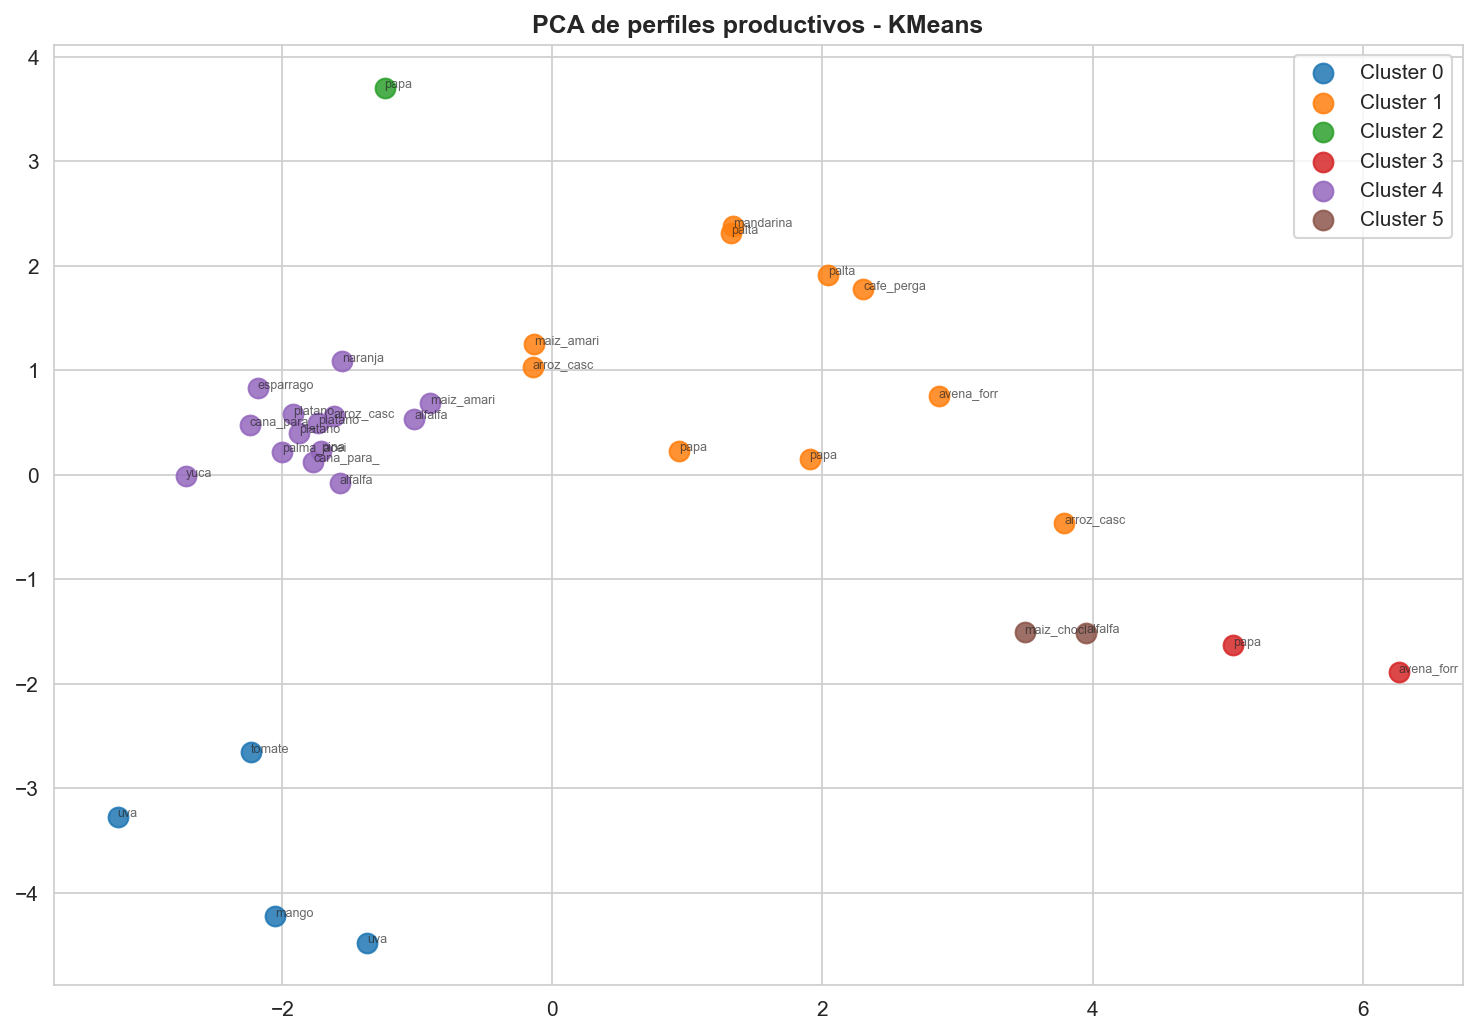
\includegraphics[width=0.46\textwidth]{06b_pca_perfiles.png}
    \caption{Modelo B: proyección PCA de los perfiles productivos coloreada por cluster.}
    \label{fig:pca_b}
\end{figure}

\subsubsection{Comparación de los tres enfoques}
La Fig.~\ref{fig:comparativa} resume la comparación. El Silhouette no es comparable directamente entre enfoques porque cada uno opera en un espacio de \textit{features} distinto: el alto valor del modelo inicial premia la redundancia geográfica. El ARI con la región es el discriminador clave: 0.59 (inicial, geografía), 0.40 (Modelo A, territorial por diseño) y 0.06 (Modelo B, patrón productivo). El ARI entre las particiones inicial y B es 0.18, confirmando que responden preguntas distintas. En síntesis, el modelo inicial promete tipificar cultivos pero tipifica regiones; el Modelo A tipifica el territorio y lo asume; el Modelo B sí tipifica cultivos por su comportamiento productivo.

\begin{figure}[h]
    \centering
    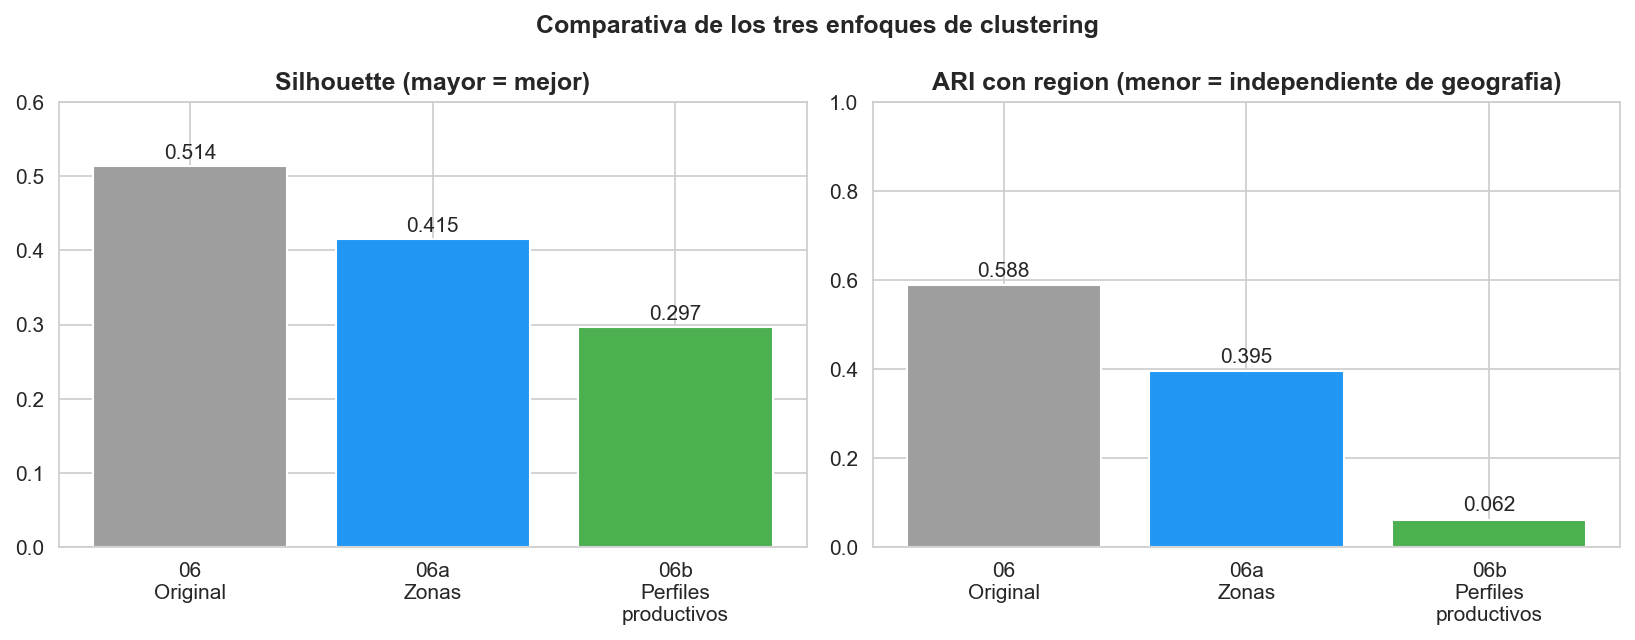
\includegraphics[width=0.48\textwidth]{comparativa_3enfoques.png}
    \caption{Comparativa de los tres enfoques. El ARI con la región revela que solo el Modelo B se independiza de la geografía.}
    \label{fig:comparativa}
\end{figure}

\section{Discusión y conclusiones}
Los resultados muestran que el agro peruano responde a dinámicas climáticas diferenciadas según el piso ecológico más que según la unidad administrativa regional. La radiación domina la estacionalidad costera, mientras que la humedad de suelo y la temperatura máxima condicionan la productividad en sierra y altiplano; en selva, la humedad relativa adquiere mayor relevancia. Estas relaciones cambian de signo entre pisos para variables equivalentes, comportamiento que permanecería oculto bajo promedios regionales.

Los eventos extremos refuerzan esta heterogeneidad. La sequía altoandina de 2022 redujo la producción agregada de Puno entre 37\% y 50\%, pero el análisis desagregado mostró impactos mucho más severos en cultivos andinos tradicionales (quinua $-64\%$, oca $-62\%$, papa $-47\%$), parcialmente amortiguados por la avena forrajera. El Fenómeno del Niño 2023--2024 produjo respuestas contrastantes: Piura con anomalías extremas de precipitación ($+121\%$) y San Martín con reducción pese al calentamiento generalizado.

La fase de modelado aporta una contribución metodológica más allá del caso peruano: demostramos que el \textit{clustering} de perfiles agroclimáticos puede reproducir trivialmente la geografía cuando las \textit{features} climáticas están degeneradas, y que métricas internas como Silhouette no detectan este sesgo. El Índice de Rand Ajustado frente a la geografía es un diagnóstico simple y efectivo. A partir de él derivamos dos modelos válidos y complementarios: tipologías territoriales (Modelo A) para caracterizar el territorio, y tipologías de patrón productivo (Modelo B) para tipificar cultivos independientemente de su ubicación.

El estudio presenta cuatro limitaciones. Primero, la asociación cultivo--distrito se construyó con criterio agronómico documentado, pero no puede validarse directamente porque MIDAGRI publica producción solo a nivel regional. Segundo, la resolución de NASA POWER ($\sim$50\,km) limita la captura de microclimas en zonas andinas de topografía compleja \cite{ramirez2012}. Tercero, el análisis se realizó en toneladas físicas y no en valor económico, subponderando cultivos de alta rentabilidad. Finalmente, los reportes del MIDAGRI contienen revisiones retroactivas sobre datos preliminares (``p/''), introduciendo incertidumbre en las series recientes; y el número reducido de unidades (33 perfiles, 12 zonas) limita el poder estadístico del \textit{clustering}, por lo que las tipologías deben leerse como exploratorias.

Como trabajo futuro, los datasets construidos permiten desarrollar modelos predictivos por cultivo--piso (Random Forest, \textit{gradient boosting}), incorporar índices ENSO y estimar impactos económicos mediante precios FOB \cite{chlingaryan2018}. La conclusión principal es que la región administrativa no constituye la unidad analítica natural del agro peruano: la heterogeneidad intra-regional exige enfoques de muestreo, análisis y modelado que respeten la estructura ecológica del territorio. Esto sugiere que las políticas agrarias frente al cambio climático deberían diseñarse por piso ecológico y patrón productivo, y no únicamente por delimitaciones regionales.

\begin{thebibliography}{00}

\bibitem{bcrp2025} Banco Central de Reserva del Perú, ``Actividad económica: Enero 2025,'' Nota de Estudios 23-2025, Mar. 2025. [Online]. Available: \url{https://www.bcrp.gob.pe/docs/Publicaciones/Notas-Estudios/2025/nota-de-estudios-23-2025.pdf}

\bibitem{adex2026} Asociación de Exportadores (ADEX), ``Adex Hoy: Agroexportaciones 2025,'' Ed. 37081, Mar. 2026. [Online]. Available: \url{https://www.adexperu.org.pe/}

\bibitem{inei2024} Instituto Nacional de Estadística e Informática, ``Encuesta Nacional Agraria,'' 2024. [Online]. Available: \url{https://www.inei.gob.pe/}

\bibitem{inia2019} H. Dorado, ``Uso de minería de datos en agricultura para hacer frente al cambio climático,'' Instituto Nacional de Innovación Agraria (INIA), 2019.

\bibitem{senamhi2009} SENAMHI, ``Impacto del cambio climático en cultivos anuales,'' 2009. [Online]. Available: \url{https://web2.senamhi.gob.pe/load/file/01401SENA-12.pdf}

\bibitem{unap2016} Universidad Nacional del Altiplano, ``Estudio agroclimatológico,'' Repositorio UNAP, 2016.

\bibitem{restrepo2017} J. M. Restrepo \textit{et al.}, ``The impact of extreme El Niño events on modern sediment transport,'' \textit{Scientific Reports}, vol. 7, no. 1, p. 11311, 2017, doi: 10.1038/s41598-017-12220-x.

\bibitem{chapapria2024} L. Chapapría and C. Viladrich, ``Modelo predictivo agroclimático usando CRISP-DM,'' Alicia Concytec, 2024.

\bibitem{canchano2024} J. C. Canchano, ``Model for demand and price prediction of agricultural products using CRISP-DM,'' in \textit{Proc. IEEE Conf. Data Mining Applications}, 2024, pp. 1--6, doi: 10.1109/ICDMMA.2024.11141314.

\bibitem{midagri2025} Ministerio de Desarrollo Agrario y Riego, ``Zonificación ecológica económica (ZEE): Suelos y aptitud agrícola,'' 2025. [Online]. Available: \url{https://www.midagri.gob.pe/portal/43-sector-agrario/suelo}

\bibitem{una2023} Universidad Nacional del Altiplano, ``Propuesta de zonificación agroecológica para el desarrollo sostenible,'' Tesis, 2023.

\bibitem{chapman2000} P. Chapman \textit{et al.}, ``CRISP-DM 1.0: Step-by-step data mining guide,'' SPSS Inc., 2000.

\bibitem{midagrihist} Ministerio de Desarrollo Agrario y Riego, ``Series históricas de producción agrícola --- hoja c-18,'' 2025. [Online]. Available: \url{https://www.midagri.gob.pe/}

\bibitem{nasa2025} National Aeronautics and Space Administration, ``NASA POWER Data Access Viewer,'' 2025. [Online]. Available: \url{https://power.larc.nasa.gov/}

\bibitem{viladrich} L. Chapapría and C. Viladrich, ``La relevancia económica de las variables climáticas en la agricultura,'' Centro de Estudios Andaluces.

\bibitem{senamhi2024} SENAMHI, ``El Niño Costero 2023--2024 fue el más intenso de los últimos 20 años en el oeste de Sudamérica,'' Abr. 25, 2024. [Online]. Available: \url{https://www.gob.pe/institucion/senamhi/noticias/944204}

\bibitem{rcr2023} Redacción RCR Perú, ``Producción agraria en Puno cayó en 70 por ciento desde el 2022 por sequía,'' Jul. 14, 2023.

\bibitem{cepiura2023} Centro de Estudios Piura, ``Estructura productiva de la región Piura,'' Gobierno Regional Piura, 2023.

\bibitem{esan2023} Universidad ESAN, ``La Libertad: ¿Cuál es su aporte a la economía exportadora del Perú?,'' 2023.

\bibitem{redesarrolloica2021} Programa Redesarrollo, ``Dato Regional Ica: Exporta de todo,'' 2021.

\bibitem{inei1996} Instituto Nacional de Estadística e Informática, ``Agropecuario: Conociendo Junín,'' 1996.

\bibitem{dataperu2021} Programa Redesarrollo, ``San Martín: Economía, salud, educación, hogares, demografía,'' DataPerú, 2021.

\bibitem{midagripuno2020} Ministerio de Desarrollo Agrario y Riego, ``Perfil productivo regional de Puno,'' 2020.

\bibitem{ramirez2012} J. Ramírez-Villegas and A. Challinor, ``Assessing relevant climate data for agricultural applications,'' \textit{Agricultural and Forest Meteorology}, vol. 161, pp. 26--45, 2012.

\bibitem{chlingaryan2018} A. Chlingaryan, S. Sukkarieh, and B. Whelan, ``Machine learning approaches for crop yield prediction and nitrogen status estimation,'' \textit{Computers and Electronics in Agriculture}, vol. 151, pp. 61--69, 2018.

\end{thebibliography}

\end{document}
